% Chapter 1

\chapter{Tube With Mixing Vanes : DEBORA-Promoteur and AGATE-Promoteur Experiments} % Chapter title

\minitoc

\label{chap:debora_agate_prom} % For referencing the chapter elsewhere, use \autoref{ch:introduction} 

\section{Introduction}

In PWR cores, the industrial geometry is tremendously complex compared to traditional experimental setup usually consisting of simple tubes such as in the DEBORA experiment (Chapter \ref{chap:debora}). Although simple geometries are absolutely mandatory for verification and validation of the multi-scale physics modeling involved in boiling two-phase flows, it would hardly suffice to be perform a full scaling of the industrial configurations. 

\npar

To that extent, there is a need for experimental measurements both in representative flow conditions \textbf{\underline{and}} geometry. This implies reproducing test sections including complicated shapes such as grids inducing significant transverse flow and turbulent mixing. 

\npar

In this Chapter, we focus on such a dedicated experiment called DEBORA-Promoteur and propose some analyses of its experimental measurements. Its single-phase counterpart called AGATE-Promoteur is also presented.



\section{DEBORA-Promoteur}
\label{sec:deb_prom_desc}

\subsection{Test Section and Experimental Campaigns}

In 2003, the wish to investigate boiling flows in complex geometries similar to those of PWR fuel assembly motivated CEA and EDF to perform modifications of the DEBORA facility \cite{falk_rapport_2002}. In order to mimic the turbulent mixing induced by the grids holding the fuel rods, a mixing device equipped with blades was built with respect to the geometrical properties of the mixing vanes of the PWR grids (Figure \ref{fig:debprom_vanes}).


\begin{figure}[!h]
\centering
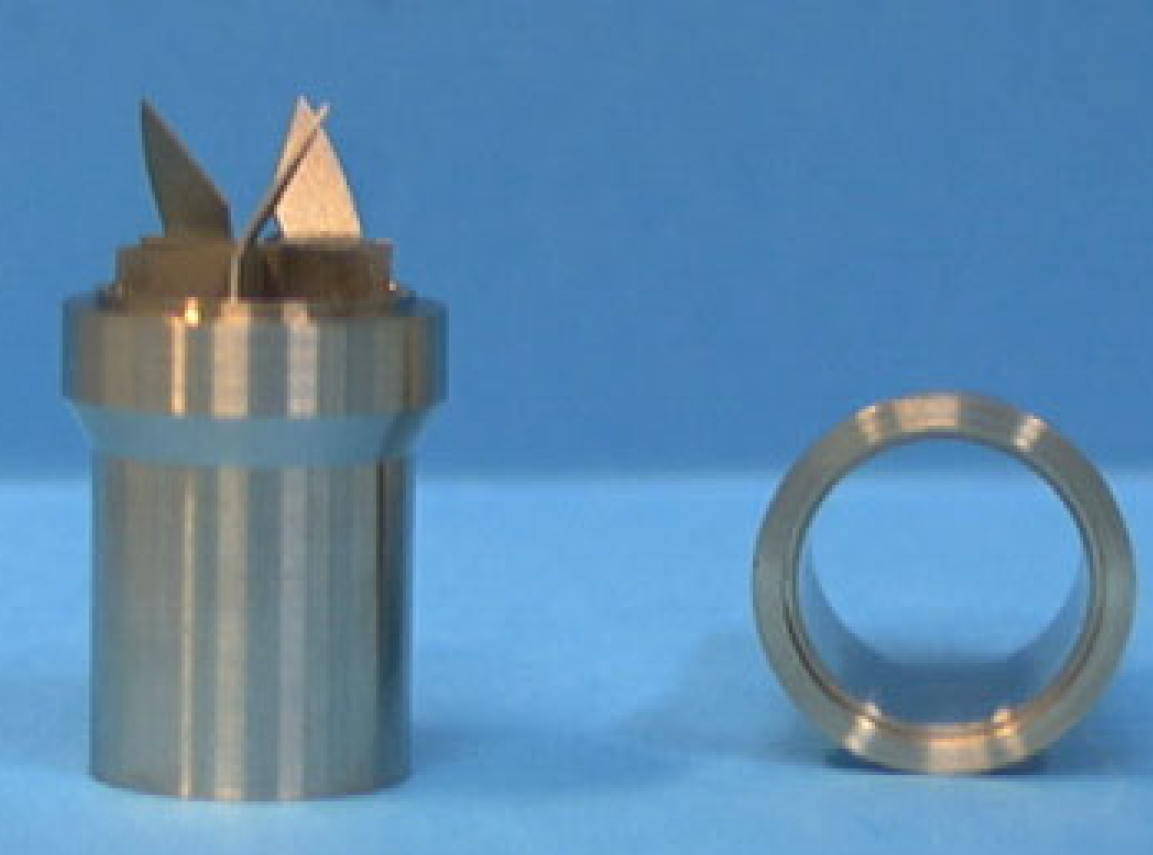
\includegraphics[width=0.3\linewidth]{img/DEBORA-Promoteur/prom_pic2.png}
\caption{Picture of the mixing device. (Adapted from \cite{falk_promoteur_2007})}
\label{fig:debprom_vanes}
\end{figure}

\npar

This mixing device was then welded into the DEBORA test section, thus named DEBORA-Promoteur. Its position upstream the end of the heating length was meant to induce a strong rotation in the flow in order to quantify the impact of the mixing regarding:

\begin{itemize}
\item Bubble recondensation for subcooled boiling ;
\item Void redistribution for saturated cases ;
\item Critical Heat Flux value compared to the naked pipe case.
\end{itemize}

Figures \ref{fig:debprom_mesrad} and \ref{fig:debprom_sketch} present the position of the measurement radius along with a sketch of the experiment, defining the position of the mixing vanes (MV) upstream the measurements section at a distance $L_{MV}$.




\begin{figure}[!h]
%%%SETTING FOR ALIGNMENT
\newlength\imageheight
%\settoheight{\imageheight}{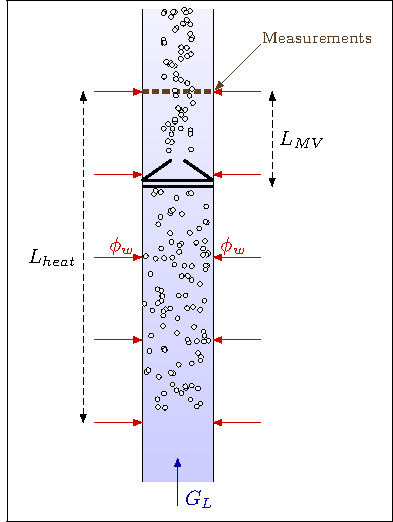
\includegraphics[width=0.45\linewidth]{img/DEBORA-Promoteur/deb_prom_sketch.pdf}}
%%%%
\centering
\subfloat[Measurement radius. (Adapted from \cite{falk_rapport_2002})]
{
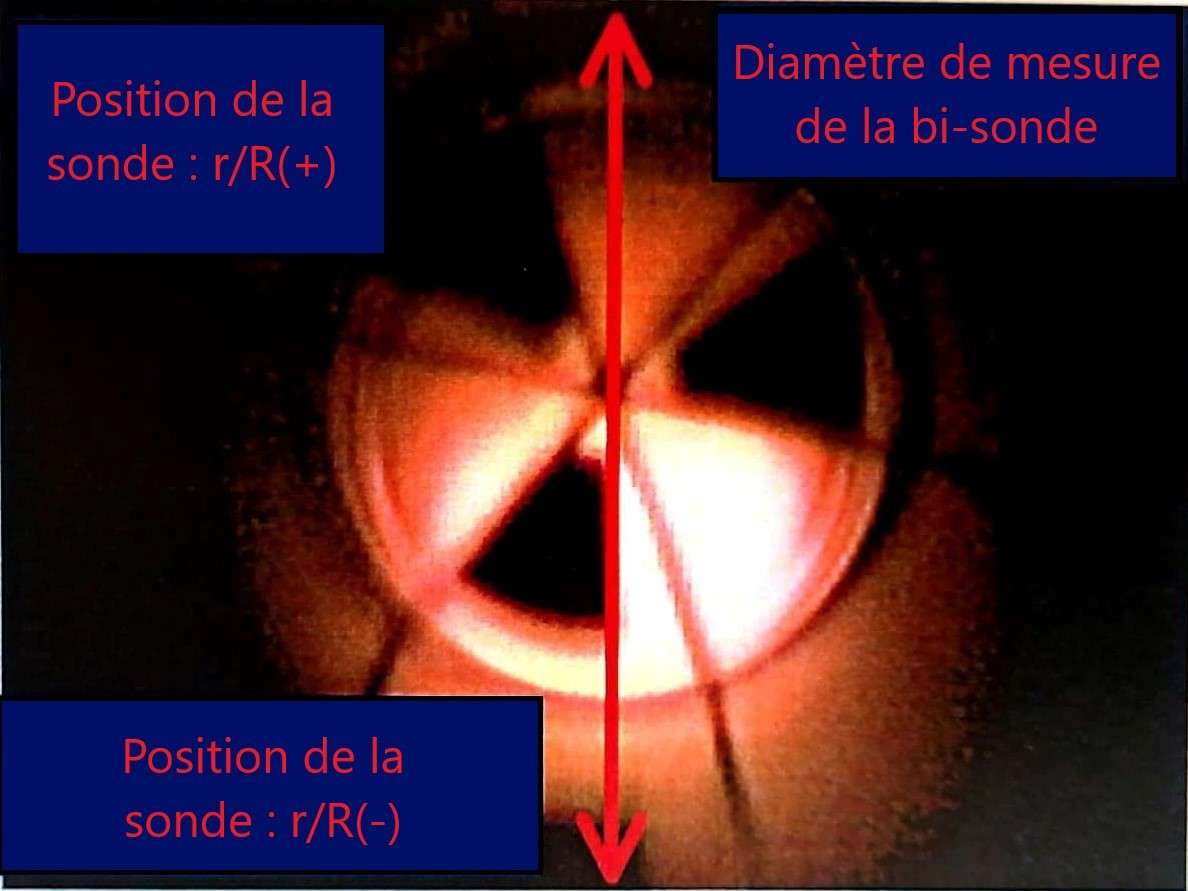
\includegraphics[width=0.3\linewidth]{img/DEBORA-Promoteur/debprom_mesrad.jpg}
\label{fig:debprom_mesrad}
}
\\
\subfloat[Sketch of the DEBORA-Promoteur test section.]{
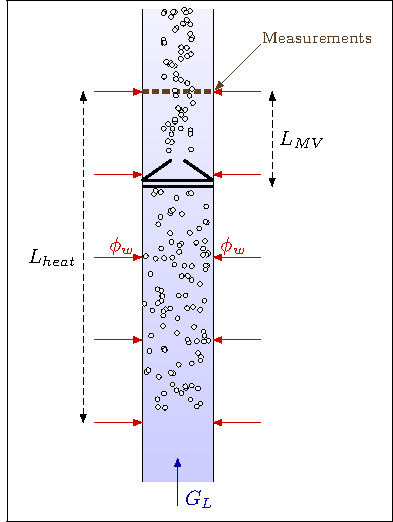
\includegraphics[width=0.45\linewidth]{img/DEBORA-Promoteur/deb_prom_sketch.pdf}
\label{fig:debprom_sketch}
}
\caption{Description of the DEBORA-Promoteur experiment.}
\label{fig:debprom_description}
\end{figure}


The same measurement instrumentation as the DEBORA C3000 cases   (bi-optical probe, Figure \ref{fig:optical_probe}) was used to study the flow topology in the DEBORA-Promoteur experiment. In that regard, two measurements campaign were conducted:

\begin{itemize}
\item Campaign C4800 where the mixing vanes were placed at $L_{MV} = 23.5\ D_{h}$ ($\approx 0.45$\ m)upstream the end of the heating length \cite{falk_rapport_2002} ;
\item Campaign C5200, where the mixing vanes were placed $L_{MV} = 10\ D_{h}$ ($\approx 0.19$\ m) upstream the end of the heating length \cite{falk_rapport_2003}.
\end{itemize}

\begin{note*}{}
Unfortunately, no thermal measurement campaign was conducted on the DEBORA-Promoteur facility.
\end{note*}

\npar


The different cases of the DEBORA-Promoteur experiment follow the same nomenclature as the DEBORA ones (Section \ref{sec:deb_exp_campaign}). A total of three test series were conducted:

\begin{enumerate}
\item Series 48G3P26WA ;
\item Series 52G3P26WA ; 
\item Series 52G3P26WB.
\end{enumerate}
where $B > A$ are the total power applied in the test section, which order of magnitude lies around those of Table \ref{tab:debora_matrix}.

\begin{note*}{}
The values of the applied heat flux for those data sets are not given in this document due to confidentiality reasons.
\end{note*}

\npar

Regarding the available data for each test, bi-optical probes allow the measurements of the void fraction but also bubble diameter using the vapor (or interfacial) velocity as explained in Subsection \ref{subsec:deb_mes_tech}. However, the measurement of the vapor velocity is reliable if:
\begin{enumerate}
\item[1)] The flow is mainly one-directional and aligned with the probles ;
\item[2)] Vapor phase is composed of spherical bubbles ;
\item[3)] Velocity gradient and center density gradient are small along a distance equal to the bubble diameter.
\end{enumerate}

Since the mixing vanes introduce a strong mixing and rotational effect, hypothesis 1) is, at first glance, impossible to verify and ensure that measurements of vapor velocity are correct. For each dataset, the available experimental file contains:

\begin{itemize}
\item 48G3P26WA: Void fraction $\alpha$ and interference frequency $\nu$ value for each probe (1 and 2)
\item 52G3P26WA \& 52G3P26WB: void fraction $\alpha$ and interference frequency $\nu$ value for each probe (1 and 2) plus the estimated (potentially uncertain) vapor velocity $U_{V,z}$.
\end{itemize}


\section{AGATE-Promoteur}
\label{sec:agate_prom_desc}

Following the DEBORA-Promoteur tests, experimental findings lead CEA and EDF to investigate the single-phase liquid velocity profile in the mixing vanes geometry, resulting in the development of an experiment called AGATE-Promoteur.

\npar

The AGATE-Promoteur experiments consist of LDV (Laser Doppler Velocimetry) measurements of the liquid velocity and turbulent intensity in both axial and radial direction. The test in conducted using the very same geometry and mixing vanes as the DEBORA-Promoteur case and consists of a single set of measurements for water at 2 bar flowing at a mass flow rate $G_{L} \approx 3000\ \debm$ (same mass flux as the DEBORA-Promoteur cases) and $T_{L} \approx 40\degC$, resulting in an hydraulic Reynolds number $\Re_{D_{h}} \approx 8.5\times 10^{4}$. Measurements are then operated at several axial positions (18) and diameters (6). Figure \ref{fig:agate_mes} details the different positions where measurements were conducted.




\begin{figure}[!h]
\centering
\subfloat[Radial measurements diameters. (Adapted from \cite{falk_promoteur_2007})]
{
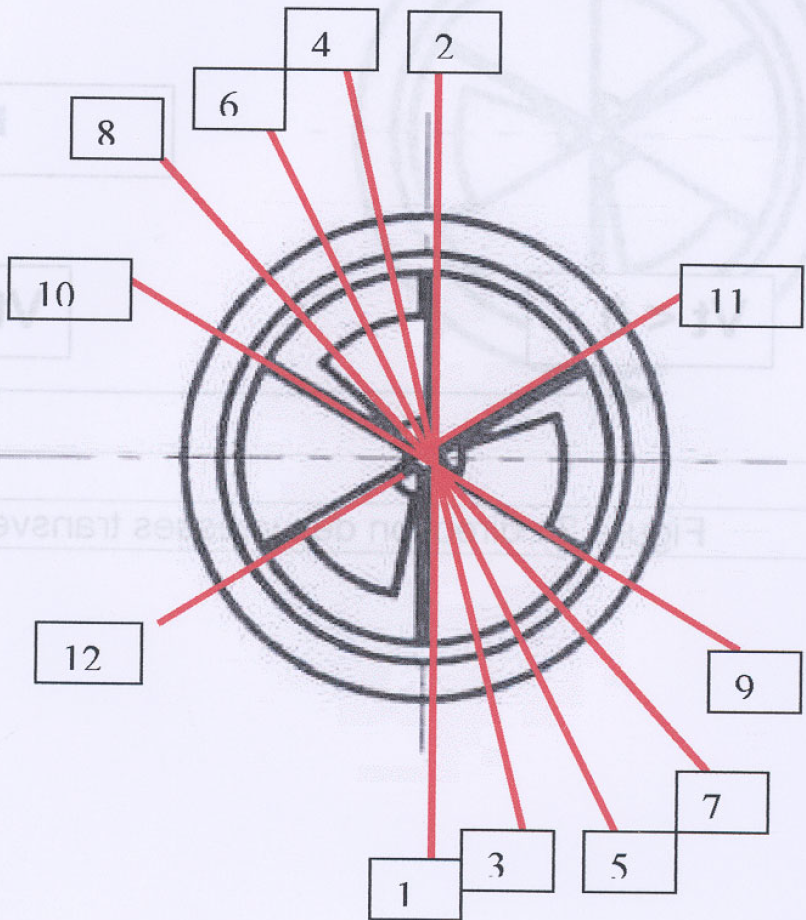
\includegraphics[width=0.3\linewidth]{img/AGATE/agate_mes_rad.PNG}
\label{fig:agate_mesrad}
}
\\
\subfloat[Axial positions of measurements.]
{
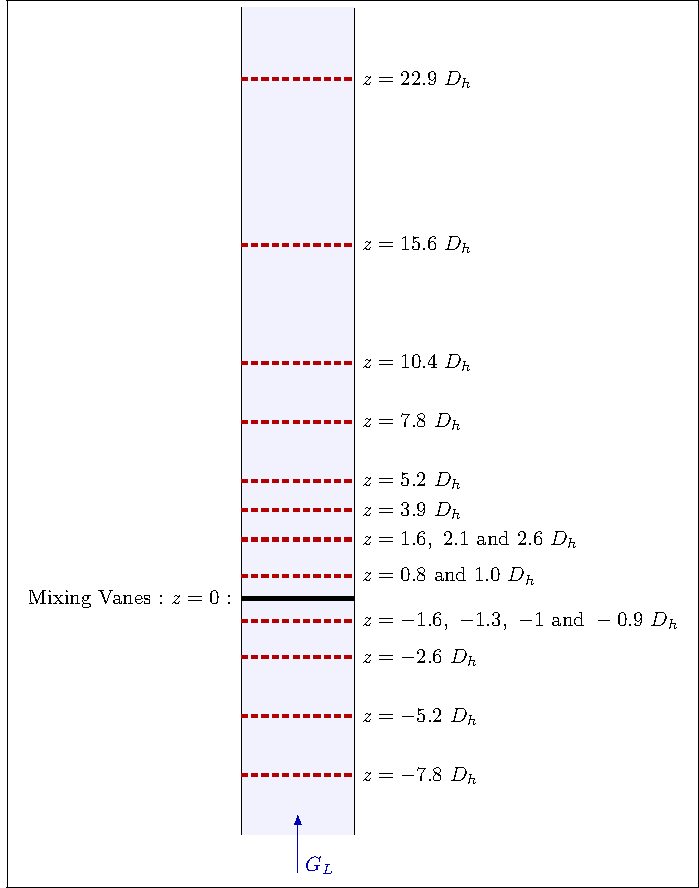
\includegraphics[width=0.45\linewidth]{img/AGATE/agate_mes_ax.pdf}
\label{fig:agate_mesax}
}
\caption{Covered measurements positions in AGATE-Promoteur experiment.}
\label{fig:agate_mes}
\end{figure}


\npar



Each diameter has 24 points of measurements, with a total of 108 diameters covered in the whole test both upstream and downstream of the mixing vanes. 

\npar

For each data point, we have the local axial velocity, radial velocity (signed positive or negative depending on its direction relative to the measured diameter), axial and radial turbulent intensities. Later, we will prefer reconstructing the values of the local RMS (Root Mean Square) of the velocity:

\begin{equation}
RMS_{i} := \sqrt{\left<U'_{i}U'_{i}\right>} = I_{T,i} \times \left<U_{i}\right>
\label{eq:RMS_def}
\end{equation}
where $i=A,\ R$ for axial or radial direction, $U=\left<U\right> + U'$ the velocity decomposed between time-average and fluctuation, and $I_{T}$ the measured turbulent intensity. 




\section{Analysis of the DEBORA-Promoteur Experimental Measurements}
\label{sec:deb_prom_anal}

On Figures \ref{fig:exp_48G3P26W23}, \ref{fig:exp_52G3P26W23} and \ref{fig:exp_52G3P26W27}, we plot respectively the void fraction and interference frequency (averaged for the two probes) for campaigns 48G3P26WA, 52G3P26WA and 52G3P26WB.



\subsubsection{48G3P26WA cases}


\begin{figure}[!h]
\centering
\subfloat[Void fraction]{
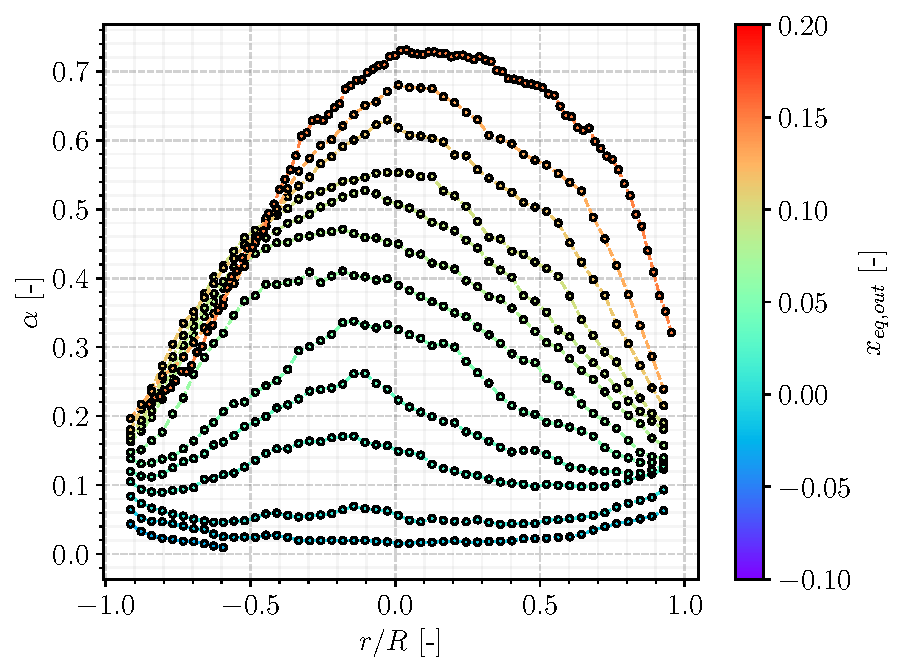
\includegraphics[width=0.5\linewidth]{img/DEBORA-Promoteur/48G3P26W23/48G3P26W23_alpha.pdf}
\label{fig:48G3P26W23_alpha}
}
\subfloat[Interference frequency]{
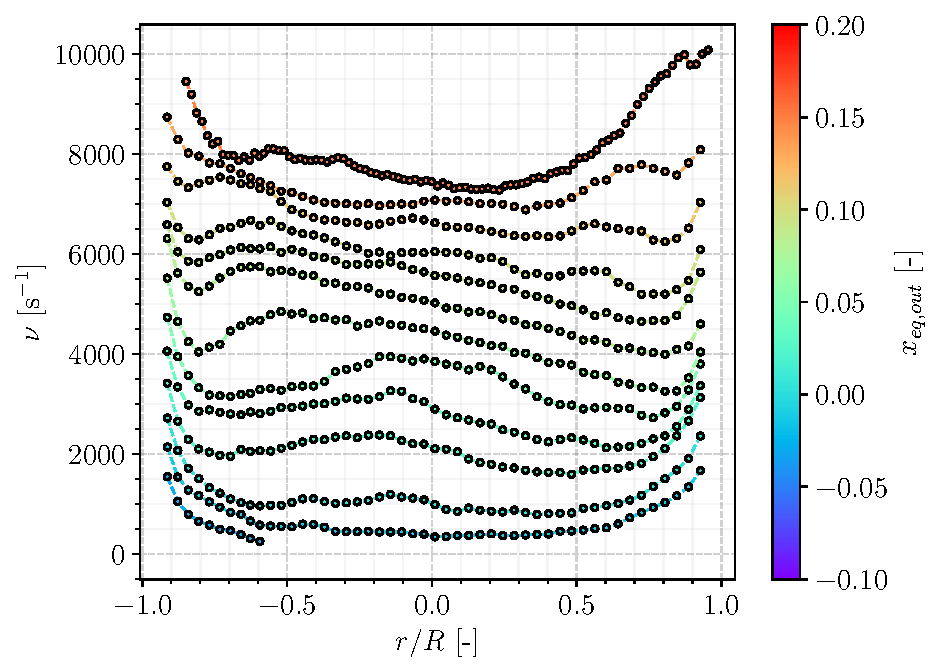
\includegraphics[width=0.5\linewidth]{img/DEBORA-Promoteur/48G3P26W23/48G3P26W23_nu.pdf}
\label{fig:48G3P26W23_nu}
}

\caption{Experimental results from the 48G3P26WA series.}
\label{fig:exp_48G3P26W23}
\end{figure}

\npar
The first immediate observation is the position of the void fraction peak positioned at the center of the tube (Figure \ref{fig:48G3P26W23_alpha}), strongly differing from the naked tube (Figure \ref{fig:G2P26W16_alpha}). This is a direct consequence of the mixing vanes inducing a rotational flow that will gather the vapor at the center. Except for lowest quality cases, the void fraction at the wall is the minimum value along the measurement radius, which insists on the inversion of the void fraction profile under the mixing vanes effect. 

Moreover, the profile is not perfectly symmetrical with a void peak progressively shifting towards positive values of $r/R$. This could be expected since the mixing vanes do not present any axisymmetry.

\npar

Analyzing the interference frequency (Figure \ref{fig:48G3P26W23_nu}), \ie the number of interface detection per second, allow to qualitatively determine whether if the measured void fraction at a given point is the result of a large number of small bubbles or a small number of large bubbles going through the probes. We note for hottest cases that the interference frequency reaches its maximum at the wall where the void fraction is the lowest, while its minimum is at the center where void fraction is maximal. This means that fewer bubbles at the center lead to a larger void fraction compared to the wall, which is likely to indicate the effect of coalescence increasing the average bubble size. 

\subsubsection{52G3P26WA and WB cases}


The main difference between the C5200 and C4800 cases is the position of the mixing vanes that are closer to the end of the mixing length in the C5200 campaigns ($10\ D_{h}$ versus $23.5\ D_{h}$).

\begin{figure}[!h]
\centering
\subfloat[Void fraction]{
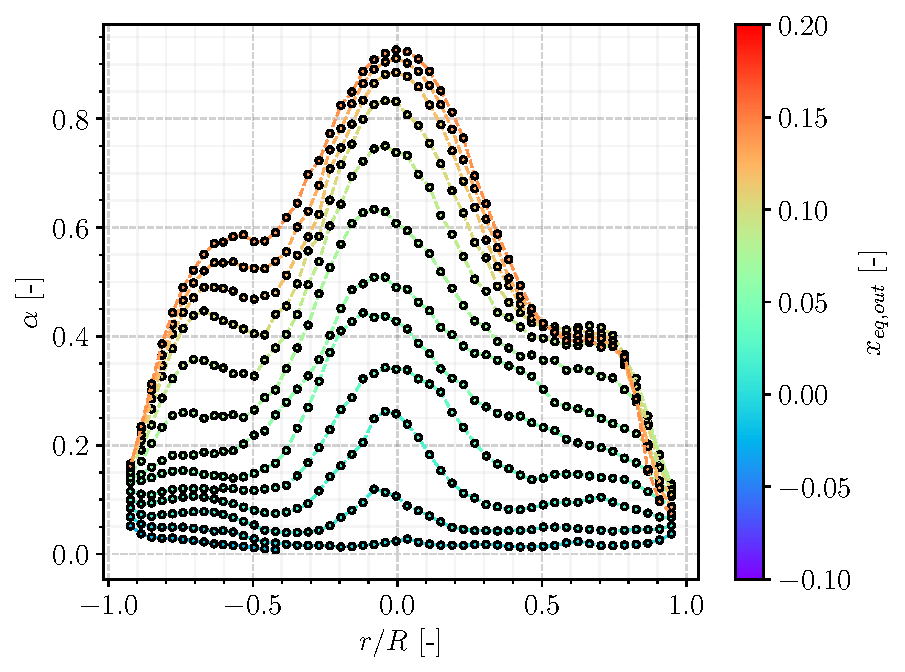
\includegraphics[width=0.5\linewidth]{img/DEBORA-Promoteur/52G3P26W23/52G3P26W23_alpha.pdf}
\label{fig:52G3P26W23_alpha}
}
\subfloat[Interference frequency]{
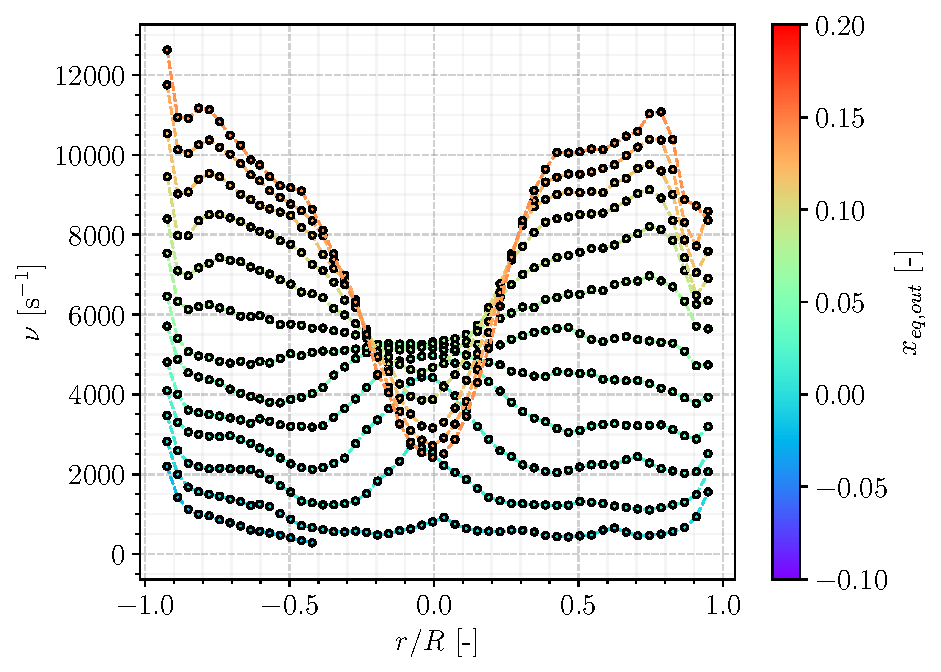
\includegraphics[width=0.5\linewidth]{img/DEBORA-Promoteur/52G3P26W23/52G3P26W23_nu.pdf}
\label{fig:52G3P26W23_nu}
}

\caption{Experimental results from the 52G3P26WA series.}
\label{fig:exp_52G3P26W23}
\end{figure}


\begin{figure}[!h]
\centering
\subfloat[Void fraction]{
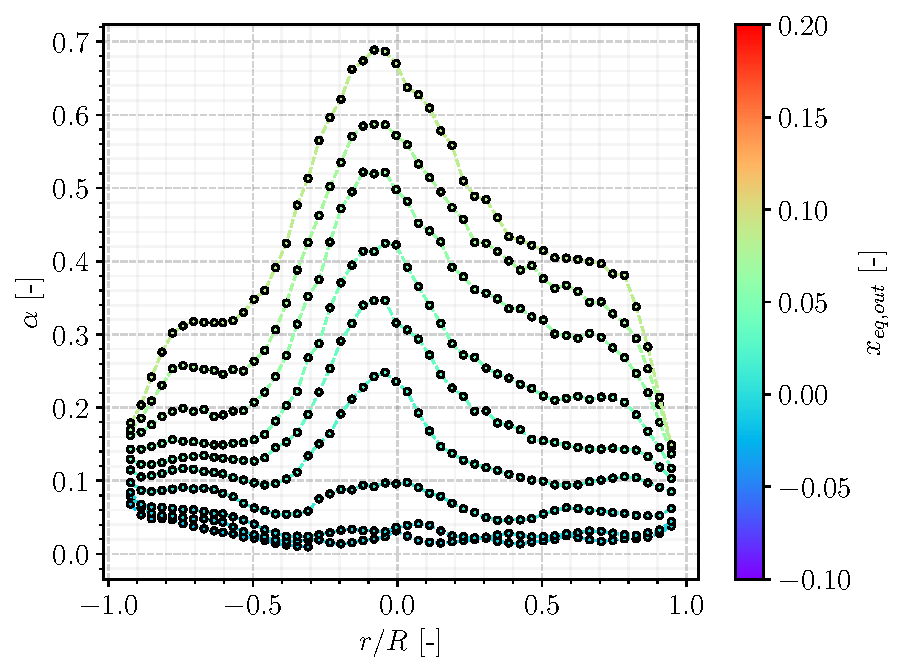
\includegraphics[width=0.5\linewidth]{img/DEBORA-Promoteur/52G3P26W27/52G3P26W27_alpha.pdf}
\label{fig:52G3P26W27_alpha}
}
\subfloat[Interference frequency]{
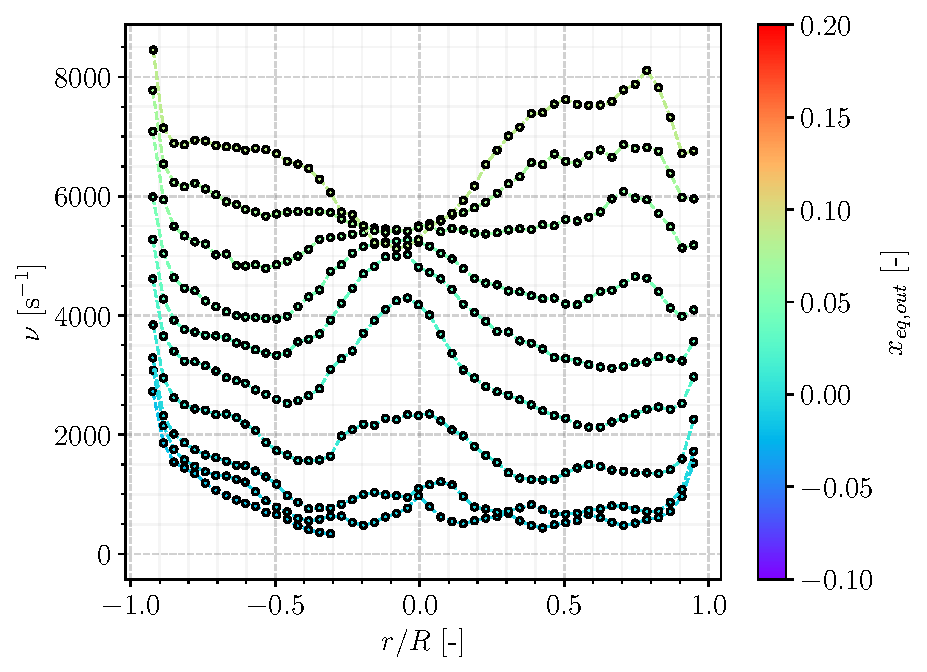
\includegraphics[width=0.5\linewidth]{img/DEBORA-Promoteur/52G3P26W27/52G3P26W27_nu.pdf}
\label{fig:52G3P26W27_nu}
}

\caption{Experimental results from the 52G3P26WB series.}
\label{fig:exp_52G3P26W27}
\end{figure}

\npar

Similar to C4800 cases, we observe a void fraction peak at the center and minimum at the wall (Figures \ref{fig:52G3P26W23_alpha} and \ref{fig:52G3P26W27_alpha}). However, the shape of the measurements largely differs by presenting local maximum values around $r/R = \pm 0.6$ for hottest cases. The void fraction peaks are also higher than for C4800 cases, with values up to $90\%$. This is probably an effect of the MV positions since moving the vanes downwards means that the flow will be mixed later, leaving a shorter distance for the flow to fall back to a traditional single tube profile. The amount of vapor suddenly brought to the center will increase as the distance between the vanes and the measurement section reduces.

\begin{remark*}{}
Such an effect may be assimilated to a so-called "history effect", meaning that the distance to such a mixing device has an impact over the two-phase flow properties.
\end{remark*}

\npar

Interference frequencies (Figures \ref{fig:52G3P26W23_nu} and \ref{fig:52G3P26W27_nu}) profiles are also differing from C4800 cases. The interference peak is initially located at the center for low quality cases, meaning that there is a larger number of bubbles at the center compared to the wall. However, the shape reverses as the outlet quality increases (and thus the core void fraction), with a huge decrease of the bulk interference frequency which significantly points towards predominant coalescence effects. Noting that this change happens roughly when $x_{eq,out} \leq 0$ (saturation is reached) indicates that it may originates from the absence of condensation.   

\begin{remark*}{}
The considerations over condensation are though speculative and would largely benefit from liquid temperature measurements in such a configuration, which could both quantify the impact of mixing on the liquid phase and correlate interference frequencies to local subcooling values.
\end{remark*}


\subsection{Estimation of the Bubble Diameter}
\label{subsec:debprom_dV_exp}

Since values of vapor velocity measurements are given for the C5200 cases, one may be interested in exploiting them to try to extract information about the bubble size distribution in the flow. However, we have to be able to tell whether those measurements were largely erroneous due to the rotation effects or not \ie if the bubbles were moving in the direction of the probes.

\npar

To do so, we propose two arguments:

\begin{itemize}
\item Analyzing the difference between the measured interference frequencies for each probe, which could help to quantify if the number of bubbles detected largely differ between them. If so, it means a strong rotation made bubbles flowing through only one probes. On the contrary, this would support the fact that, locally, bubbles were globally flowing in the direction of the probes.

\item Quantifying the importance of the radial velocity compared to the axial velocity in the measurement section.
\end{itemize}


On Figure \ref{fig:exp_C52_deltanu}, we plot the relative difference of interference frequency between the two probes for each C5200 campaign. 


\begin{figure}[!h]
\centering
\subfloat[52G3P26WA series]{
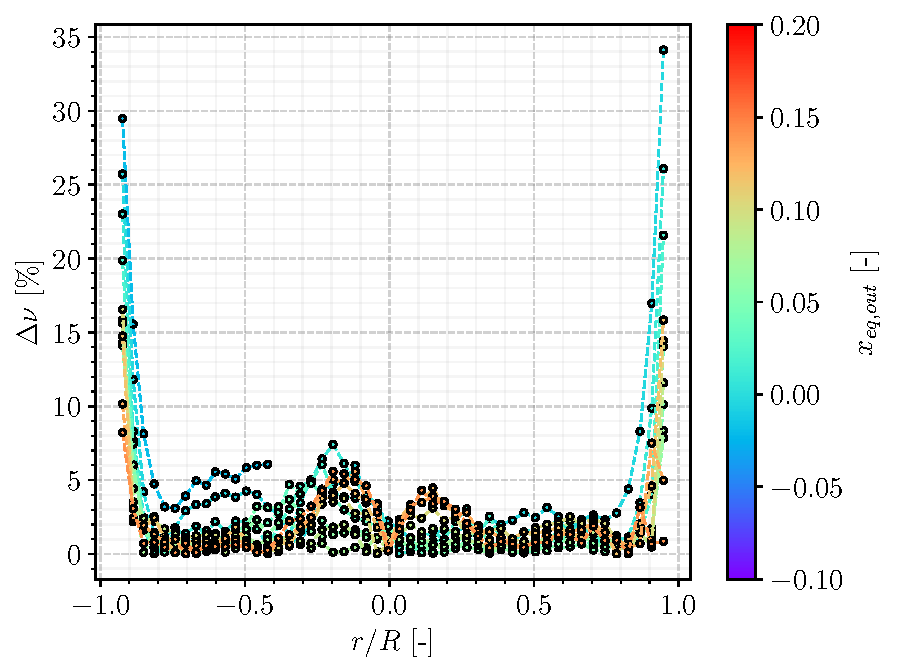
\includegraphics[width=0.5\linewidth]{img/DEBORA-Promoteur/52G3P26W23/52G3P26W23_deltanu.pdf}
}
\subfloat[52G3P26WB series]{
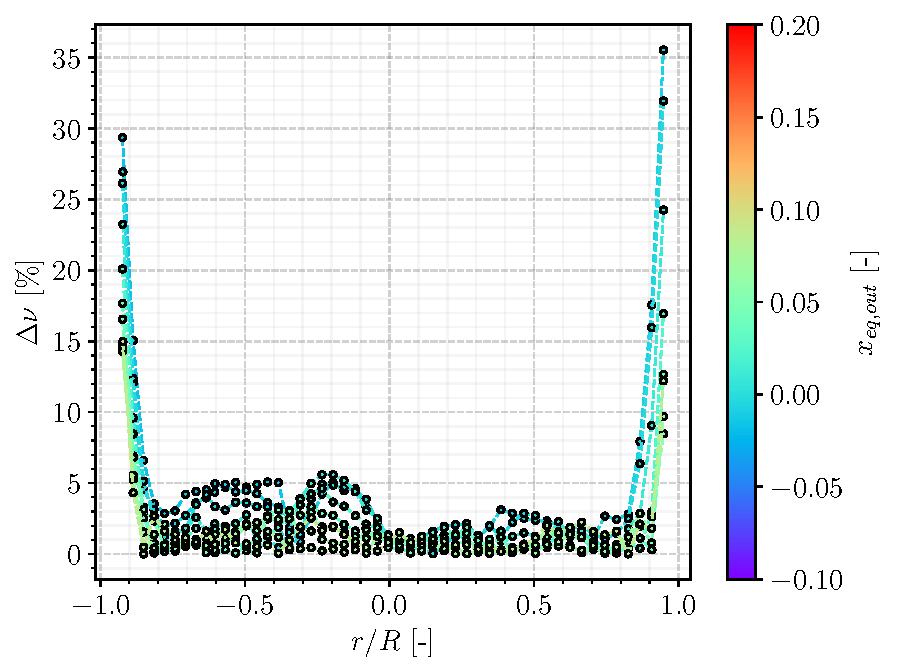
\includegraphics[width=0.5\linewidth]{img/DEBORA-Promoteur/52G3P26W27/52G3P26W27_deltanu.pdf}
}

\caption{Relative difference of interference frequency for the two probes.}
\label{fig:exp_C52_deltanu}
\end{figure}


\npar


We see that, close to the wall, the interface detection of the probes differ by up to 35\%, which clearly indicates a vapor phase moving radially. However, as we approach the center ($-0.75 \leq r/R \leq 0.75$), the difference in interference frequency globally falls below $5\%$, potentially showing that bubbles at those locations were having mostly axial velocities.

\npar

To quantify the importance of the radial velocity at the measurement section ($z\approx 10\ D_{h}$ after the grids), we rely on the AGATE-Promoteur experimental results (Section \ref{sec:agate_prom_desc}). Based on the different measured diameters at each axial position, we can compute the average value of the ratio between radial and axial velocities $U_{R} / U_{A}$ depending on the height $z$. The results are shown on Figure \ref{fig:exp_agate_Urap_z}


\begin{figure}[!h]
\centering
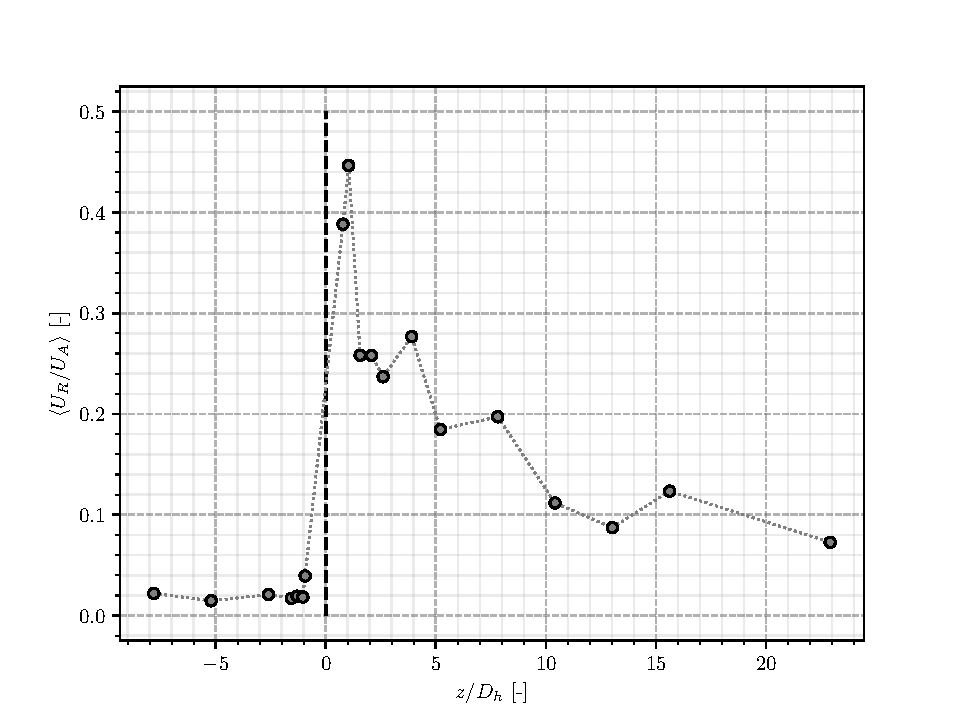
\includegraphics[width=0.6\linewidth]{img/AGATE/Urap_z.pdf}
\caption{Average relative importance of radial velocity to axial velocity in AGATE-Promoteur experiment. Black dotted lines denotes the position of the MV.}
\label{fig:exp_agate_Urap_z}
\end{figure}


\npar

The mixing effect on liquid velocity is clear: the average induced rotation velocity can reach up to 45\% of the axial velocity in the section right after the MV. The importance of the radial velocity then naturally fades with the distance to the MV, becoming of the order of $10\%$ at $z\approx 10\ D_{h}$. 

\npar

At the position corresponding to the measurements in the C5200 campaign, the radial velocity then is approximately 10 times smaller than the axial velocity. This comforts the fact that the flow direction is mainly axial when the measurement using the bi-optical probe is conducted.

\npar

Altogether, those two analyses both support the fact that the hypothesis of a flow aligned with the probes at $z=10\ D_{h}$ downstream the MV is reasonable. Therefore, we allow ourselves to use the measured values of the vapor velocity $U_{V,z}$ \textbf{\underline{between $r/R=-0.75$ and $r/R=0.75$}} in the C5200 cases to propose \textbf{\underline{an estimation}} of the bubble diameter in DEBORA-Promoteur measurements:

\begin{equation}
D_{V} \approx \frac{6 \alpha U_{V,z}}{4\nu}
\end{equation}


Resulting values are presented on Figure \ref{fig:exp_C52_dvap}.

\begin{figure}[!h]
\centering
\subfloat[52G3P26WA series]{
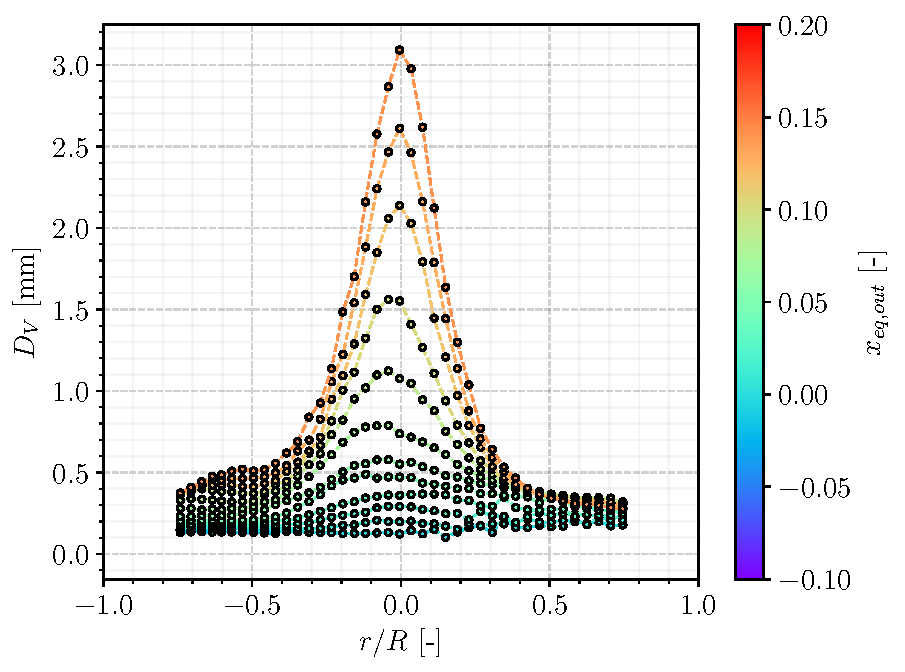
\includegraphics[width=0.5\linewidth]{img/DEBORA-Promoteur/52G3P26W23/52G3P26W23_dv.pdf}
}
\subfloat[52G3P26WB series]{
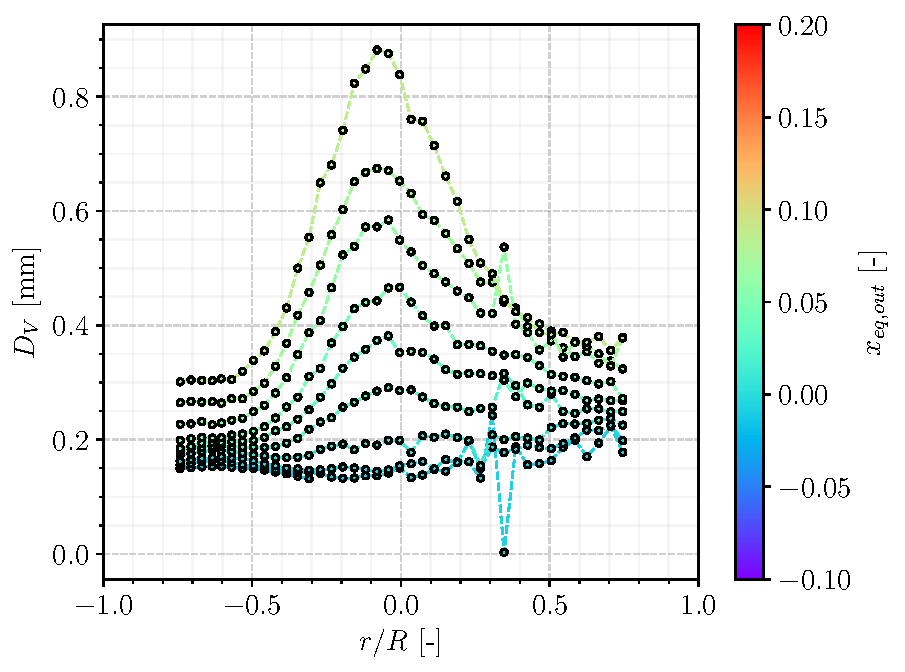
\includegraphics[width=0.5\linewidth]{img/DEBORA-Promoteur/52G3P26W27/52G3P26W27_dv.pdf}
}

\caption{Estimation of bubble diameter on C5200 measurements series.}
\label{fig:exp_C52_dvap}
\end{figure}

\npar

First, we notice that the values attained closer to the wall mostly lie between 0.1\ mm and 0.5\ mm which is coherent with the values observed in the naked tube case (Figure \ref{fig:G2P26W16_dv}).

\npar

When approaching the center of the pipe for high qualty cases, the bubble diameter sharply increase with values that can reach up to 3\ mm. In those conditions, such a diameter is the result of an important coalescence along with negligible condensation effects. Although very large void fractions are reached, those bubble diameters are still an order of magnitude lower than the tube diameter meaning we are not in presence of a slug or annular flow at the center. The resulting flow regime at high void fractions is likely looking like a foam composed of several millimeters bubbles separated by thin layers of liquid.

\begin{remark*}{}
In such two-phase flow conditions, the dispersed approach is unlikely to be representative of the real physics at stake. Strong interaction between the bubbles can be expected. %and the nearly absence of liquid means it can not be considered as the leading fluid anymore.

\npar

Moreover, the optimal packing for non-overlapping spheres of same sizes is mathematically capped at 74\% \cite{wu_bulk_2003}, bubbles at void fraction $\alpha > 74\%$ then must have, at least partially, non-spherical shapes. Which is also supported by Weber number value $\We \sim 0.1$ and E\"otv\"os value $\Eo \sim 1$ in those conditions.
\end{remark*}

%Wu, Yugong; Fan, Zhigang; Lu, Yuzhu (1 May 2003). "Bulk and interior packing densities of random close packing of hard spheres". Journal of Materials Science. 38 (9): 2019–2025. doi:10.1023/A:1023597707363. ISSN 1573-4803. S2CID 137583828.


\section{Conclusions}

The analysis of the DEBORA-Promoteur experiment allowed to qualitatively qualify the two-phase flow in a geometry including mixing vanes. So far, we can remember that:

\begin{itemize}
\item The mixing vanes have a clear impact on the vapor distribution, gathering it at the center of the tube thus reversing the radial void fraction profile.

\item The axial distance to the mixing vanes appears to have a significant influence over the vapor distribution, further enlightening the presence of a "history effect". 

\item An estimation of the bubble diameter in those conditions was achievable and showed very important coalescence effects with bubble diameters increasing up to 10 times larger when moving from the wall to the center. \textbf{This constitutes a new element of analysis of the DEBORA-Promoteur tests.}

\item Void fraction can reach very high values with peaks at the center up to $90\%$, which combined with the bubble diameter value indicates that the flow may look like a foam composed of vapor bubbles with thin layers of liquid between them.
\end{itemize}


In the next chapter, we perform numerical simulations of the DEBORA-Promoteur and AGATE-Promoteur experiments to assess NEPTUNE\_CFD capacity on such geometries.